\chapter{Introduction}
\label{intro}
Leukaemia is a cancer of the hematopoietic system, and is classified according to the affected cell lineage and according to its rate of development, thus \textit{acute myeloid leukaemia} refers to a particularly aggressive and rapidly proliferating class of leukaemia which affects the myeloid cell line. This occurs when undifferentiated myeloid cells called myeloblasts acquire mutations which hinder further differentiation but allow for their rapid clonal proliferation \citep{Khwaja2016}. The causative genetic or cytogenetic abnormalities which induce cancer are expressed in the cell's transcriptome, which can be quantified into discrete transcripts using RNA sequencing (RNA-seq). 

RNA-seq is the application of \ac{NGS} techniques to measure the quantity of RNA sequences in a biological sample, in a given moment \citep{zhong2009}. It has gradually replaced microarrays as the standard method of measuring a cell's RNA profile, offering less technical noise, high throughput of transcriptomic data, and a lower overall cost for the mapping of large transcriptomes \citep{zhao2014comparison, rao2019comparison}. 

In this dissertation we will use this technology to detect whether a phenolic treatment was successful in inducing differentiation in HL-60 cells, an \ac{AML} cell-line. If differentiation can be induced in \ac{AML}, the undifferentiated myeloid cells will be forced to take an epigenetic path (e.g. towards becoming a monocyte), culminating in apoptosis \citep{santos2000expression, mark2017transcriptomes}. This fundamental transformation of the cells is reflected in their transcriptome. A 'snapshot' of the cell's transcriptomes will be taken at three time-points (1hr, 6hr, 12hr) after the administration of the treatment, which will be compared to the transcriptome of a fourth sample, the negative control (which may be regarded as the time-point '0hr') through differential gene expression analysis. If the treatment was successful, we should expect to see differential expression in genes involved in pathways related to apoptosis, cancer and differentiation.



\section{Motivation} 
Despite incremental improvements in treatment over the past few decades, average \ac{AML} 5-year survival rates remain at 28\% for affected individuals, which decreases with age and unfavourable cytogenetics, according to the SEER database \citep{sasaki2021novo}. Chemotherapy is currently standard practice for the treatment of \ac{AML}, despite its indiscriminate cytotoxic effects and resultant physiological consequences on the patient. As a result of their frail state, older adults usually cannot withstand the side-effects of this treatment and are instead put under palliative care with abysmal chances of even short-term survival \citep{lancet2018overall}. 

Recent decades have seen rapid progress in high-throughput sequencing techniques and our understanding of cancer biology, which have lead to the development of novel targeted treatments. One of these relatively recent approaches is differentiation therapy, where a pharmacological agent encourages differentiation in cancer cells. This alters the cancer's immature, stem-cell like state, halting its ability to rapidly proliferate and metastasise. The differentiation agent \ac{ATRA} has been particularly successful in treating the \ac{AML} subtype of acute promyelocytic leukaemia (APL), managing to achieve a 90\% survival rate, while avoiding the severe cytotoxic side-effects of chemotherapy \citep{kim2015selection}. This dissertation is an attempt to use recent developments in RNA-seq technology to potentially identify a similarly acting compound to further increase our arsenal in our war against cancer, specifically against \ac{ATRA}-resistant strains of \ac{AML}, whilst sparing the patient of the severe side-effects associated with chemotherapy.


\section{An Introduction to RNA-seq}

The specifics of the RNA-seq workflow are highly variable, with many competing techniques for many steps in the process currently in use. A generic representation of the wet-lab processes involved can be seen in Figure \ref{fig:rnaseq_biorender}. An essential step common to every workflow is the extraction of RNA from the sample tissue or cells. This is a particularly tricky endeavour as RNA is chemically unstable due to the hydroxyl groups at the 2' and 3' positions, facilitating RNase activity (RNA-degrading enzymes) \citep{green2019win}. This issue is compounded by the ubiquity and chemical resilience of RNAses, meaning that special care must be taken to avoid contamination of glassware and instruments that interact with the RNA \citep{green2019win}. The sample is lysed to extrude the contents of the cell, and DNA and proteins are removed via phase separation between two immiscible liquids. The end result should be the high-quality RNA in an aqueous solution. The resulting RNA is composed of messenger RNA (mRNA), transfer RNA (tRNA) and various other categories of non-coding RNA (ncRNA), most notably ribosomal RNA which makes up 95\% of the total RNA and is irrelevant to our analysis \citep{kukurba2015rna}. This bulky rRNA is removed using oligo-dT primer beads or commercially available kits specific to the removal of rRNA \citep{peano2013efficient}. The next chronological step is library preparation, where RNA strands are fragmented, converted to their complimentary DNA (cDNA) strands and ligated to adapter sequences \citep{zhong2011high}. This adapter-ligated cDNA library is typically attached to a flow-cell, amplified and sequenced in a high-throughput sequencing platform which typically results in a FASTQ \citep{cock2010sanger} file. % Include more detail here?
This contains the nucleotide sequence of the cDNA in a text-based format. Each nucleotide base call is also assigned an ASCII character as a quality score. Phred quality scores are among the most widely used, which are numerical scores generally ranging from 10 to 60, logarithmically related to the probability of an erroneous base-call, represented as a single ASCII character \citep{ewing1998base}.

\begin{figure}[ht!]
  \centering
  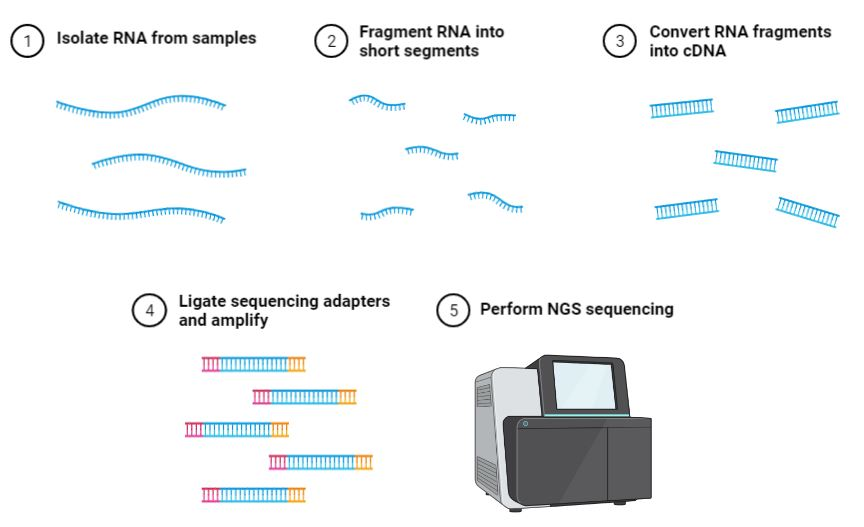
\includegraphics[width=0.9\linewidth]{rnaseq_biorender}
  \caption[Summary of the wet-lab processes which occur prior to RNA-seq data analysis.]{Summary of the wet-lab processes which occur prior to RNA-seq data analysis. Created using \href{https://biorender.com/}{BioRender.com}.}
  \label{fig:rnaseq_biorender}
\end{figure}

This brings us to the part of RNA-seq which was performed during this dissertation: the data analysis. This involves the construction of a pipeline consisting of multiple tools stitched together with the aim of gaining insight on the differentially expressed genes between samples. As a result of the decentralised nature of bioinformatics, and the potential variability of the data and goals of the researcher, there is no one-size-fits-all tool. The researcher constructing the pipeline must take into account a myriad of trade-offs for each tool for each step of the pipeline. However the steps to an RNA-seq pipeline protocol can be generalised as:
\begin{enumerate}
\item \textbf{Quality Control} - This involves the visualisation of the sequencing data to assess its quality, identifying any potential sequencing errors. This step translates the quality scores embedded in FASTQ files into something more interpretable such as a line graph. Other common quality metrics may include GC content, the number of \textit{N} symbols and presence of adapter sequences. Recognising certain patterns in data quality visualisation is essential to identifying the source of the problem \citep{stoler2021sequencing}.
\item \textbf{Preprocessing} - This is an optional step performed only if \ac{QC} indicates that there are issues with the data. Adapter sequences, low-complexity regions and low Phred scores are considered \textit{low-quality}, thus have a high probability of being erroneous and are discarded \citep{martin2011cutadapt, prinseq++}. Other metrics (e.g. GC content) are harder to amend, and may be indicative of a deeper problem further upstream in the process. 
\item \textbf{Alignment} - Reads are compared to a reference genome or reference transcriptome and aligned to the regions of highest similarity. Aligners typically first find an exact match between the two, which they use as a \textit{seed}. The seed is extended through an implementation of dynamic programming to find the optimal alignment.
\item \textbf{Quantification} - This step produces a gene count matrix containing the number of reads which fall within the coordinates of a particular gene. Typically, the row names would be gene IDs and column names would be the sample IDs, with each cell representing the number of reads which fall within that gene region.
\item \textbf{Normalisation} - Confounding variables which are not biologically relevant and induce differences between samples and between genes must be accounted for for an unbiased comparison of samples. The main factors to account for are sequencing depth \citep{robinson2010scaling}, gene length \citep{oshlack2009transcript} and GC content \citep{risso2011gc}. This step may be fused with the previous or following one depending on the tool. 
\item \textbf{Differential Expression} - Statistical tests are performed to see whether a significant difference exists between the normalised sample read counts and a benchmark sample considered to be 'normal' or 'healthy'. Every compared gene typically produces two values: the $log_{2}$ fold-change (logFC) and the p-value (adjusted for multiple testing). A threshold is applied to each of these to determine which genes should be considered as differentially expressed. If the logFC is positive, the gene is up-regulated, while if it is negative, the gene is considered down-regulated when compared to the benchmark sample.
\item \textbf{Downstream analysis} - Typically involves some form of visualisation of the \ac{DEG} to gain biological insight, but further analysis depends greatly on the research question. Possible routes are gene expression clustering, pathway analysis and functional term over-representation analysis \citep{conesa2016survey, chung2021best}.
\end{enumerate}

\section{Aim and Objectives} 
\label{Aim and Objectives}
This dissertation shall be performing RNA-seq analysis on data generated during a PhD thesis by \cite{Gatt2016}. During this preliminary study, an \ac{ATRA}-resistant HL-60 cell line was used to model \ac{AML}, and was treated with a phenolic mixture across four time-points (further detail in the Section \ref{method:prelim study}). The general aim of this dissertation is to provide insight into the molecular mechanism of differentiation caused by the phenol treatment on the \ac{ATRA}-resistant HL-60 cells over time through bulk RNA-seq analysis. To achieve this, six objectives must be attained:

\begin{enumerate}
\item Determine which bioinformatics tools are best suited to be used in this RNA-seq pipeline given the current data
\item Perform quality control checks on the data files at various stages of analysis to identify and adjust poor quality data
\item Assign genes to each read through the alignment to a recent human reference genome or transcriptome release
\item Conduct differential expression analysis between the treated samples and the untreated control
\item Annotate, visualise and interpret the gene expression data in its biological context to provide insight into which gene-sets are being affected by the phenol treatment over time
\end{enumerate}


%\begin{figure}[ht!] % supposedly places it here ...
%  \centering
%  
\includegraphics[width=0.6\linewidth]{test_image_goku}
%  \caption[This is the short caption for List of Figures]{A test figure.  This caption is huge, but in the list of figures only the smaller version in the square brackets will appear.\index{Goku il-king}}
%  \label{fig:test1}
%\end{figure}
%A test figure is shown in Figure~\ref{fig:test1}.

%\begin{figure}[!ht]
%    \centering
%    \subbottom[Goku]{
\includegraphics[width=0.3\textwidth]{test_image_goku}}\qquad
%    \subbottom[More Goku]{
\includegraphics[width=0.3\textwidth]{test_image_goku}}%
%    \caption[Short Caption]{The same super saiyan. Two times.} 
%  \label{fig:test2}
%\end{figure}

%Two figures shown side by side are shown in Figure~\ref{fig:test2}.

\section{Our Approach}
The first step to achieve the stipulated aim was a thorough literature review to become acquainted with commonly used tools in RNA-seq analysis and their respective limitations and trade-offs. This allowed for the identification of the optimal tools suited for our dataset, which can be described as a time series with four time points, with a single sample per time point.

FastQC is an essential starting point in any Omic data analysis, due to its provision of extensive quality metrics. FastQScreen \citep{wingett2018fastq} added another layer of information by checking the sequences against multiple reference genomes, human and non-human, to check for contamination. Cutadapt \citep{martin2011cutadapt} was used to trim adapter sequences and short reads. Prinseq++ \citep{prinseq++} was then used to remove ambiguous reads and regions of low-complexity. The trimmed and filtered FASTQ files were aligned to the GRCh38.p13 reference genome \citep{ref} using the \ac{STAR} aligner \citep{Dobin2013}. \ac{STAR} was called through RSEM \citep{li2011rsem}, which after alignment, estimates gene and isoform expression levels. 

The four gene count files, containing the gene IDs and expected read counts, were imported into R \citep{R} to follow the edgeR \citep{edger} workflow, including \ac{TMM} normalisation. A negative control sample (which may be referred to as the '0 hour' time point) was used as the baseline to which the three other time points where compared to in a pairwise comparison fashion. Due to budget constraints, there were a lack of replicates in this study. While a common and often unavoidable consequence of the high costs associated with RNA-seq experiments, severely restricted the possible options for differential expression analysis. The statistical tests used by the leading \ac{DGE} tools edgeR and DESeq2 \citep{love2014moderated} both require the estimation of dispersion, which cannot be calculated using a single sample. As a workaround, the edgeR vignette\footnote{https://www.bioconductor.org/packages/release/bioc/vignettes/edgeR/inst/doc/edgeRUsersGuide.pdf} suggests an approximated value for the Biological Coefficient of Variation (BCV) based on similar studies, from which we can derive the dispersion. This approach, although inaccurate, was deemed as the most suitable method of \ac{DGE} given this dataset. These \ac{DEG}s were annotated and visualised for an overview of the differences between the samples, particularly how the transcriptome of the untreated samples changed over time with treatment. Pathway analysis was performed with a particular focus on those infamously deranged by cancer to gain further biological insight on the differentiation process occurring.

% Revisit this part later

\section{Document Structure}
This chapter has provided a surface-level introduction to the theory behind this project, why it was undertaken and what it hopes to achieve.

In the following chapter, the \textbf{Background and Literature Overview} we will delve deeper into what is currently known about \ac{AML} and RNA sequencing techniques. It will provide an overview of the relevant literature, in particular recent studies which made use of RNA-seq analysis pipelines, and how their methods and findings influenced this project.

\textbf{Methodology} will focus on the work done to achieve the aforementioned aim and objectives. We will summarise the preliminary wet-lab work performed by Dr Vassallo Gatt  \citep{Gatt2016}, and describe in detail the steps taken to construct the RNA-seq pipeline to transform the data in four FASTQ files.

In the \textbf{Results \& Discussion}, we will present the outputs of the steps described in the previous chapter, followed by a detailed interpretation. will describe the reasoning behind the construction of the RNA-seq pipeline, and justify the choice of tools and their chosen parameters. It will also compare and contrast our results with the results of previous literature, particularly the top \ac{DEG}s and deranged pathways found in this study, with those associated with \ac{AML}. 

The final chapter, the \textbf{Conclusion}, will revisit the aim and objectives and discuss if there were achieved to a satisfactory degree. Here we will give a final summary of our interpretation of the results, what could have been improved, and proposals for future work on the topic.

